\chapter{Индексы}

\begin{epigraphs}
\qitem{<<Ну у вас и запросики>> сказала база данных и зависла}{интернет}
\end{epigraphs}

Что такое таблица в реляционной СУБД? Это такой список из кортежей (tuple). Каждый кортеж состоит из ячеек (row). Количество ячеек в кортеже и их тип совпадают со схемой колонки, нескольких колонок. Этот список имеют сквозную нумерацию RowId~--- порядковый номер. Таким образом, таблицы можно осознавать как список пар (RowId, Кортеж).

Индексы~--- это обратные отношения (Кортеж, RowId). Кортеж обязан содержать больше равно одной ячейки (т.е. быть построенным минимум по одной колонке). Для индексов, которые индексируют более одной колонки~--- они ещё называются составными, и участвуют в отношениях вида <<многие-ко-многим>>~--- всё написанное верно в равной степени. Очевидно, если кортеж~--- не уникален (в колонке существует два одинаковых кортежа), то эти отношения выглядят как (Кортеж, Список RowId)~--- т.е. кортежу сопоставляется список RowId.

Индексы могут использоватся для таких операций в базе данных:

\begin{itemize}
  \item Поиск данных~--- абсолютно все индексы поддерживают поиск значений по равенству. А B-Tree~--- по произвольным диапазонам;
  \item Like~--- B-Tree и Bitmap индексы можно использовать для ускорения префиксных Like-предикатов (вида abc\%);
  \item Оптимизатор~--- B-Tree и R-Tree индексы представляют из себя гистограмму произвольной точности;
  \item Join~--- индексы могут быть использованы для Merge, Index алгоритмов;
  \item Relation~--- индексы могут быть использованы для операций except/intersect;
  \item Aggregations~--- индексы позволяют эффективно вычислять некоторые агрегационные функции~--- COUNT, MIX, MAX, а также их DISTINCT версии;
  \item Grouping~--- индексы позволяют эффективно вычислять группировки и произвольные агрегационные функции (sort-group алгоритм);
\end{itemize}




\section{Типы индексов}

В зависимости от структуры, используемой в реализации индексов, существенно различаются поддерживаемые операции, их стоимости, а также свойства читаемых данных. Давайте рассмотрим какие существуют типы индексов в PostgreSQL.


\subsection{B-Tree}

B-Tree (Boeing/Bayer/Balanced/Broad/Bushy-Tree) называют упорядоченное блочное дерево. Узлы в дереве представляют из себя блоки фиксированного размера. У каждого узла фиксированные число детей. Структура B-Tree представлена на рисунке~\ref{fig:btree_index}.

\begin{figure}[ht!]
  \center{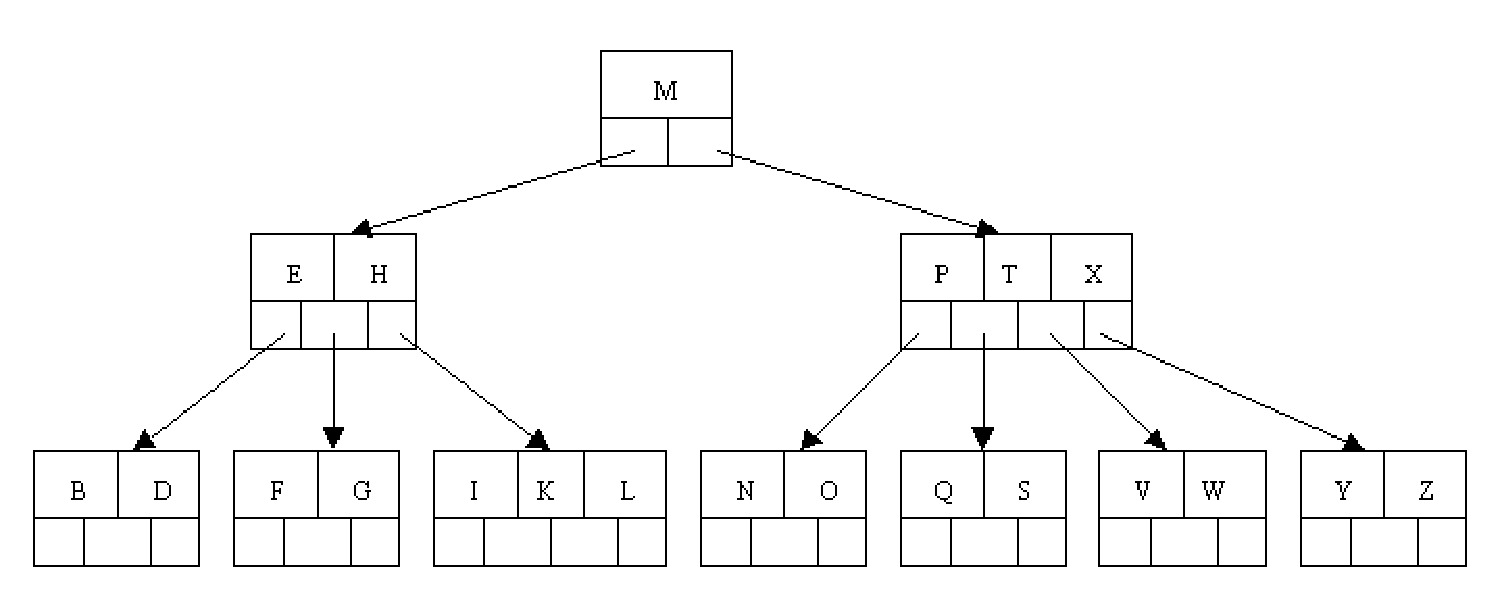
\includegraphics[width=1\textwidth]{btree_index.pdf}}
  \caption{B-Tree индекс}
  \label{fig:btree_index}
\end{figure}

B-Tree для индексов отличается от представленной на Википедии~--- есть дублированные данных в промежуточных блоках. Для i-ой записи в блоке сохраняется не значение, которое больше максимума i-го поддерева, и меньше минимума (i+1) поддерева, а максимум i-го поддерева. Различия проистекают из того, что википедия приводит пример B-Tree для множества, а нам нужен ассоциативный массив.

В индексном B-Tree значения и RowId размещаются совместно на нижнем слое дерева. Каждый узел дерева представляет из себя одну страницу (page) в некотором формате. В начале страницы всегда идёт некоторый заголовок. Для корневого и промежуточного узла в страницах хранятся пары (Значение, Номер страницы). Для листовых~--- пары (Значение ,RowId) либо (Значение, Список RowId) (в зависимости от свойств значения~--- уникально или нет). B-Tree деревья имеют крайне маленькую высоту~--- порядка $H = \log_m{N}$, где m~--- количество записей в блоке, N~--- количество элементов. B-Tree деревья являются упорядоченными~--- все элементы в любой странице (блоке) дерева лежат последовательно. Предыдущие два свойства позволяют крайне эффективно производить поиск~--- начиная с первой страницы, половинным делением (binary search) выделяются дети, в которых лежат границы поиска. Таким образом, прочитав всего H, 2H страниц мы находим искомый диапозон. Важным ньюансом является также факт, что страницы в листьях связаны в односвязный либо двусвязный список - это означает, что выполнив поиск, мы можем дальше просто последовательно читать страницы, и эффективность чтения большего объёма данных (длинного диапазона) сравнима с эффективностью чтению данных из таблицы.

Сильные стороны B-Tree индексов:

\begin{itemize}
  \item сохраняют сортированность данных;
  \item поддерживают поиск по унарным и бинарным предикатам (\lstinline!<a; = b; >c and <d; <e and >f!) за O($\log_m{N}$), где m~--- количество записей в блоке, N~--- количество элементов;
  \item позволяют не сканируя последовательность данных целиком оценить cardinality (количество записей) для всего индекса (а следовательно таблицы), диапазона, причём с произвольной точностью. Посмотрели корневую страницу~--- получили одну точность. Посмотрели следующий уровень дерева~--- получили точность получше. Просмотрели дерево до корня~--- получили точное число записей;
\end{itemize}

Слабые стороны B-Tree индексов:

\begin{itemize}
  \item для их построения требуется выполнить полную сортировку пар (Значение, RowId);
  \item занимают много места на диске. Индекс по уникальным Integer-ам к примеру весит в два раза больше аналогичной колонки (т.к. храняться ещё и RowId);
  \item при постоянной записи дерево разбалансируется, а также начинает хранить данные разреженно (сразу после построения они могут лежать очень плотно), и время доступа увеличивается за счёт увеличения объёма дисковой информации. Поэтому B-Tree индексы требуют присмотра и периодического перепостроения (REBUILD);
\end{itemize}



\subsection{R-Tree}

R-Tree (Rectangle-Tree) предназначен для хранения пар (X, Y) значений числового типа (например, координат). По способу организации R-Tree очень похоже на B-Tree. Единственное отличие~--- это информация, записываемая в промежуточные страницы в дереве. Для i-го значения в узле мы B-Tree мы пишем максимум из i-го поддерева, а в R-Tree~--- минимальный прямоугольник, покрывающий все прямоугольники из ребёнка. Подробней можно увидеть на рисунке~\ref{fig:rtree_index}.

\begin{figure}[ht!]
  \center{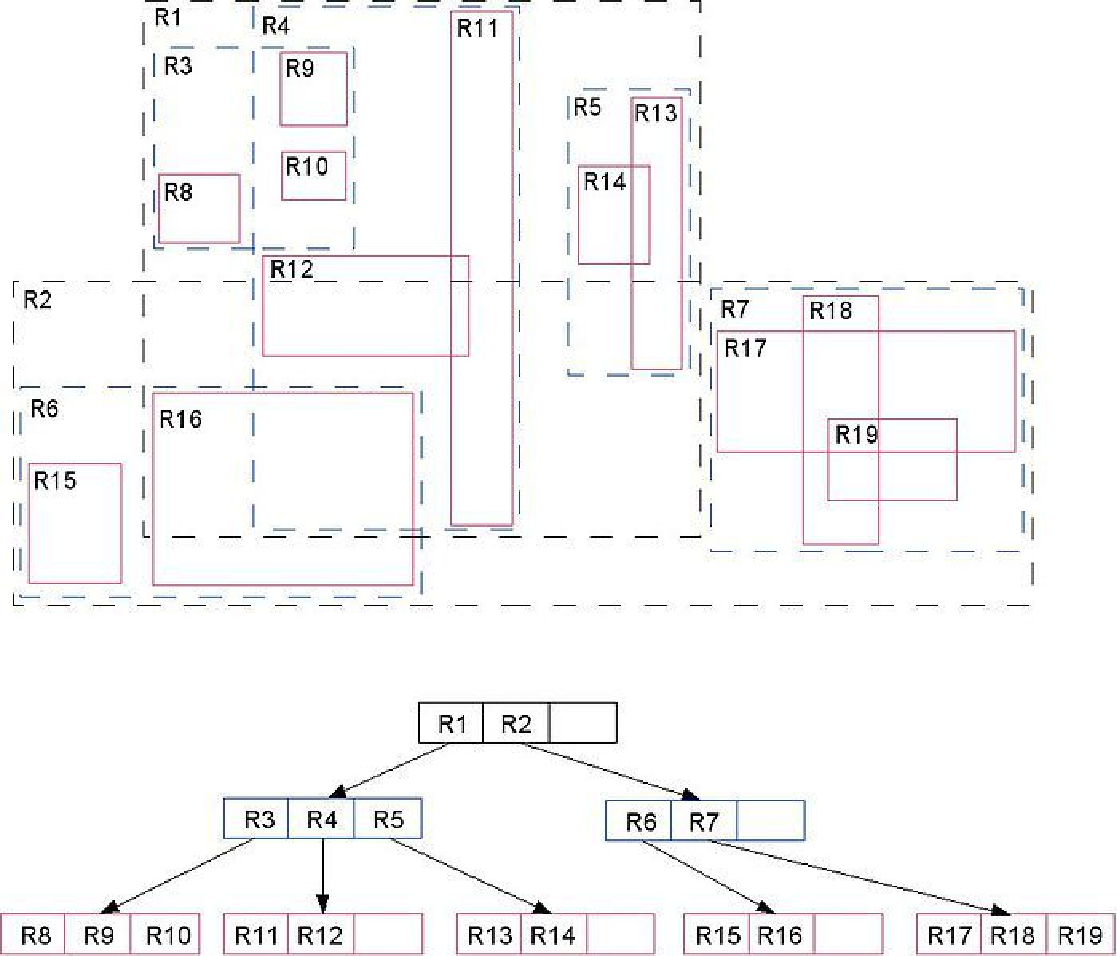
\includegraphics[width=1\textwidth]{rtree_index.pdf}}
  \caption{R-Tree индекс}
  \label{fig:rtree_index}
\end{figure}

Сильные стороны:

\begin{itemize}
  \item поиск произвольных регионов, точек за O($\log_m{N}$), где m~--- количество записей в блоке, N~--- количество элементов;
  \item позволяет оценить количество точек в некотором регионе без полного сканирования данных;
\end{itemize}

Слабые стороны:

\begin{itemize}
  \item существенная избыточность в хранении данных;
  \item медленное обновление данных;
\end{itemize}

В целом, плюсы-минусы очень напоминают B-Tree.




\subsection{Hash индекс}

Hash индекс по сути является ассоциативным хеш-контейнером. Хеш-контейнер~--- это массив из разряженных значений. Адресуются отдельные элементы этого массива некоторой хеш-функцией которая отображает каждое значение в некоторое целое число. Т.е. результат хеш-функции является порядковым номером элемента в массиве. Элементы массива в хеш-конейтнере называются букетами (bucket). Обычно один букет~--- одна странца. Хеш-функция отображает более мощное множество в менее мощное, возникают так называемые коллизии~--- ситуация, когда одному значению хеш-функции соответствует несколько разных значений. В букете хранятся значения, образующие коллизию. Разрешение коллизий происходит посредством поиска среди значений, сохранённых в букете.

\begin{figure}[ht!]
  \center{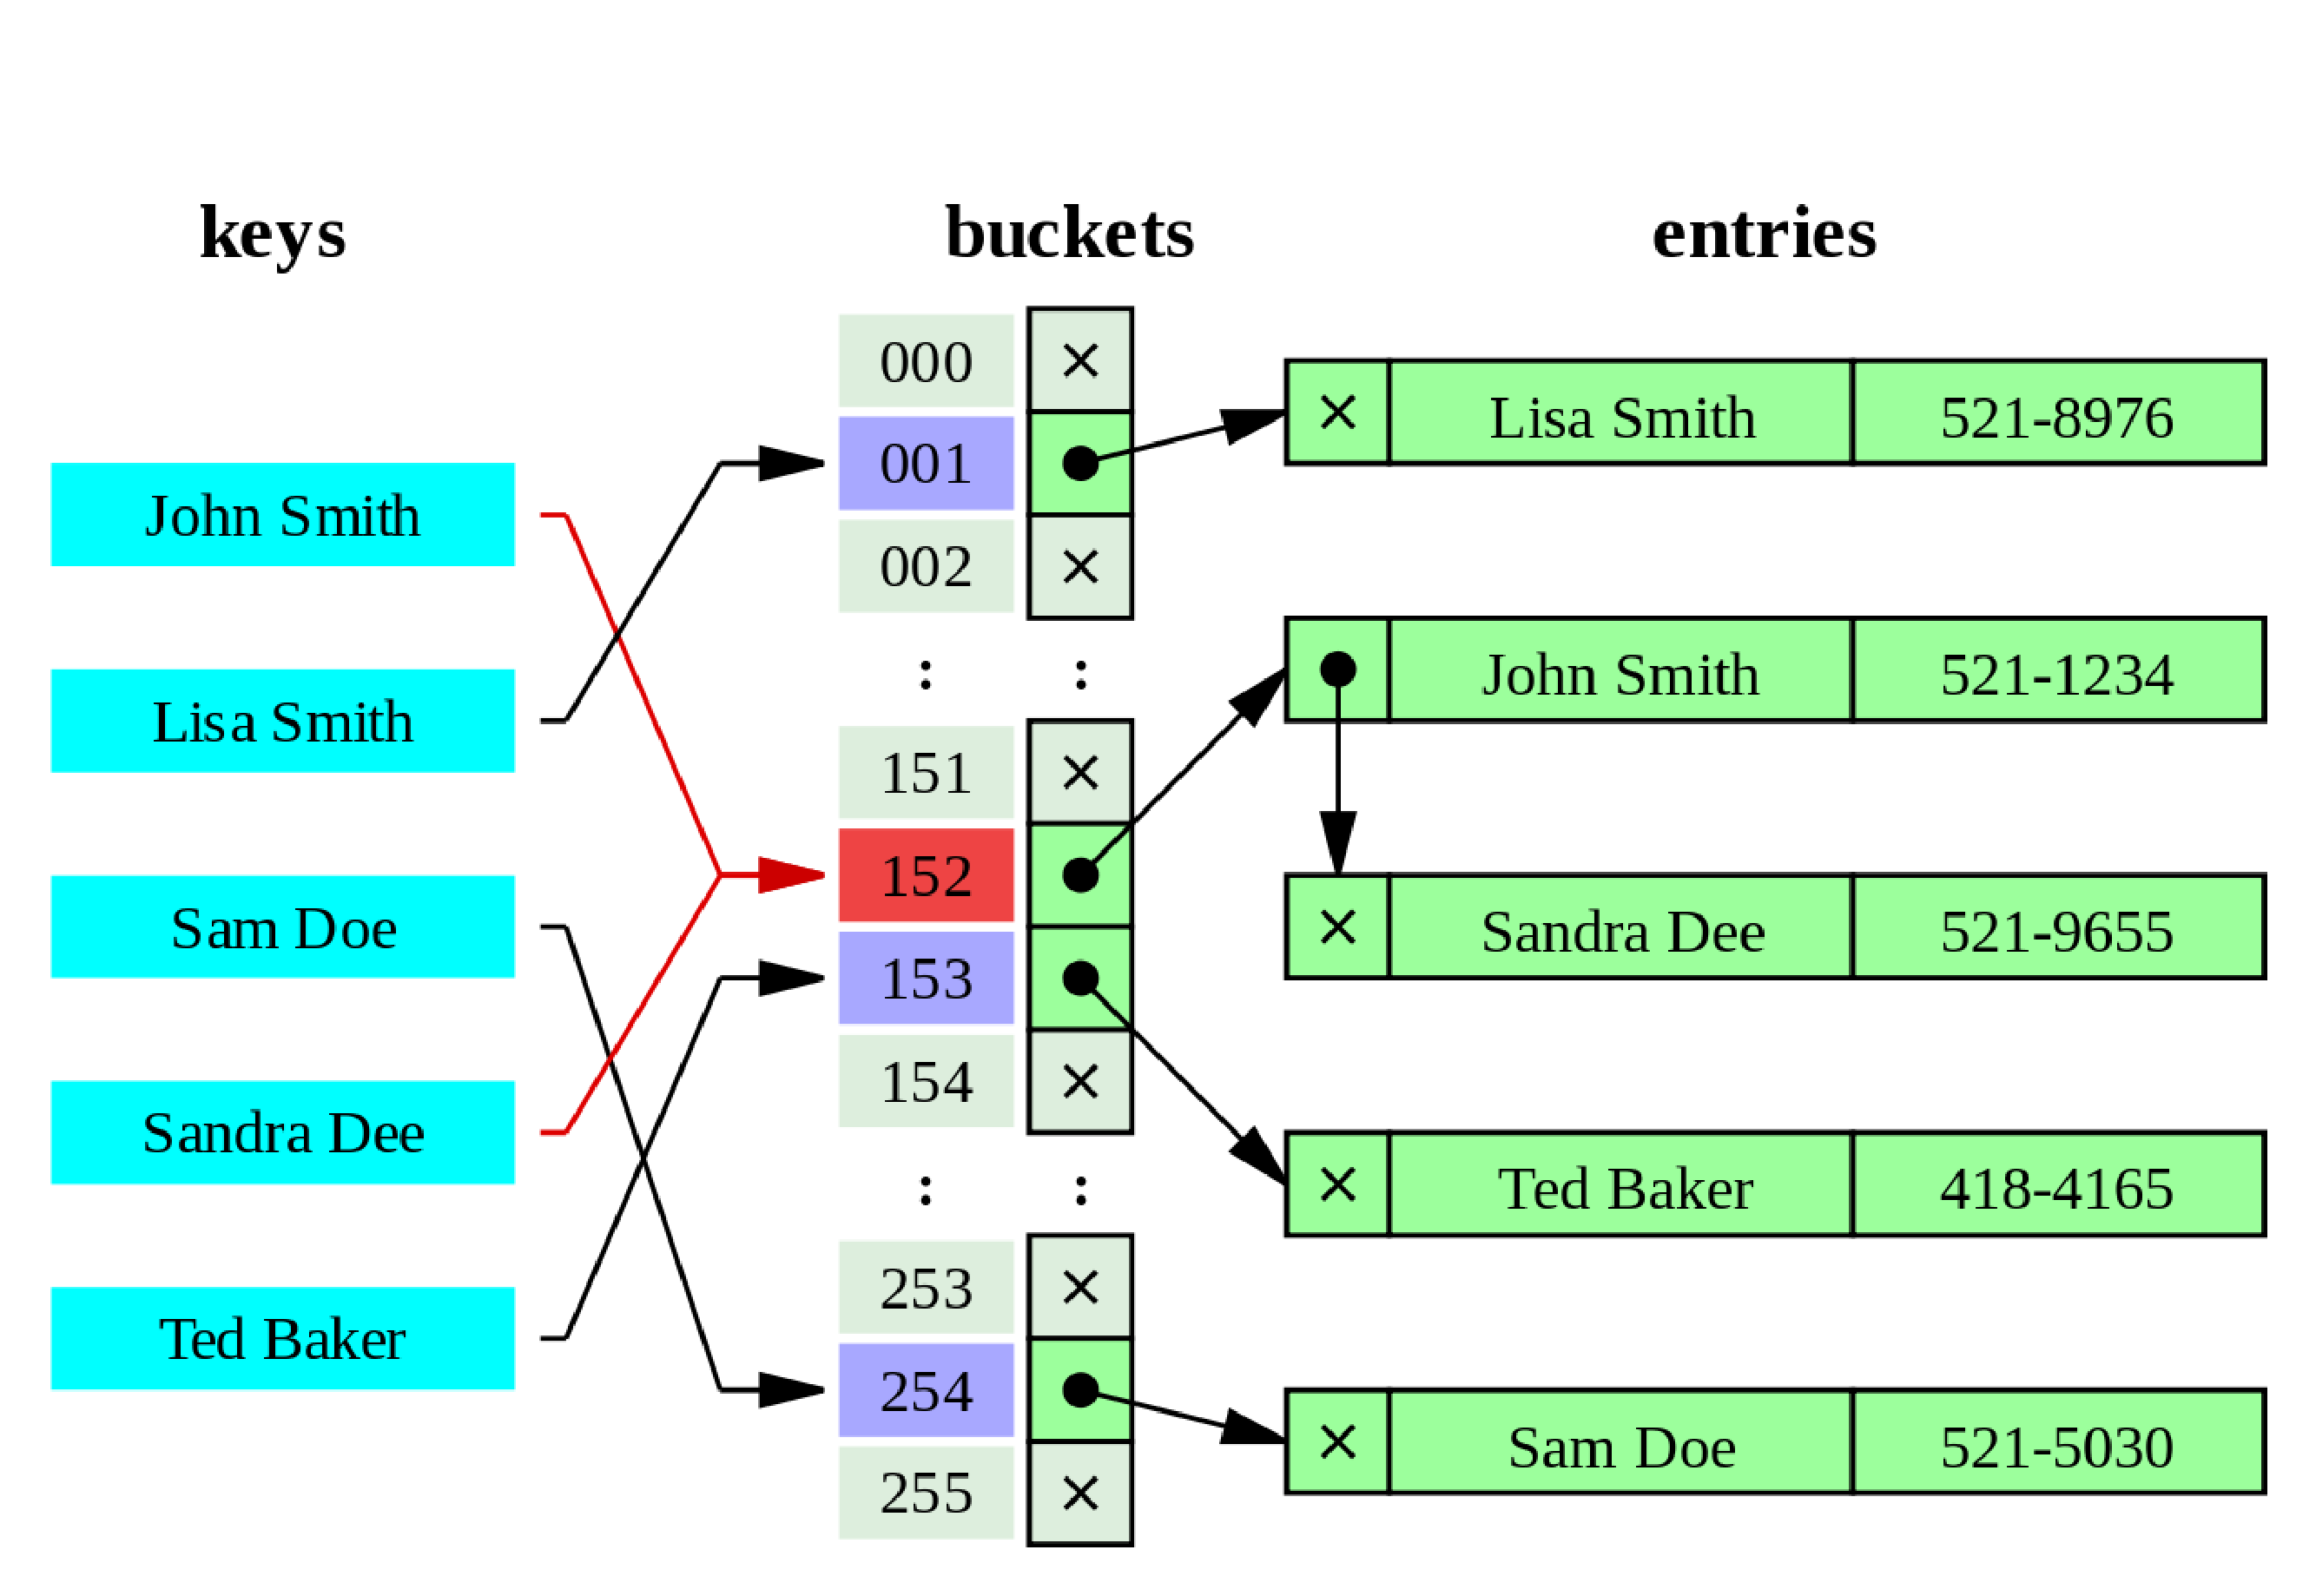
\includegraphics[width=1\textwidth]{hash_index.pdf}}
  \caption{Hash индекс}
  \label{fig:hash_index}
\end{figure}

Сильные стороны:

\begin{itemize}
  \item очень быстрый поиск O(1);
  \item стабильность~--- индекс не нужно перестраивать;
\end{itemize}

Слабые стороны:

\begin{itemize}
  \item хеш очень чувствителен к коллизиям хеш-функции. В случае <<плохого>> распределения данных, большинство записей будет сосредоточено в нескольких букетах, и фактически поиск будет происходить путем разрешения коллизий;
  \item из-за нелинейнойсти хэш-функций данный индекс нельзя сортировать по значению, что приводит к невозможности использования в сравнениях больше/меньше и <<IS NULL>>;
  \item данный индекс в PostgreSQL транзакционно не безопасен, нужно перестраивать после краха и не реплицируется через потоковую (streaming) репликацию;
\end{itemize}




\subsection{Битовый индекс (bitmap index)}
\label{sec:indexes-bitmap-index}

Битовый индекс (bitmap index)~--- метод битовых индексов заключается в создании отдельных битовых карт (последовательность 0 и 1) для каждого возможного значения столбца, где каждому биту соответствует строка с индексируемым значением, а его значение равное 1 означает, что запись, соответствующая позиции бита содержит индексируемое значение для данного столбца или свойства (\href{https://ru.wikipedia.org/wiki/%D0%9A%D0%BE%D0%B4_%D0%A5%D0%B0%D1%84%D1%84%D0%BC%D0%B0%D0%BD%D0%B0}{алгоритм Хаффмана}).

\begin{figure}[ht!]
  \center{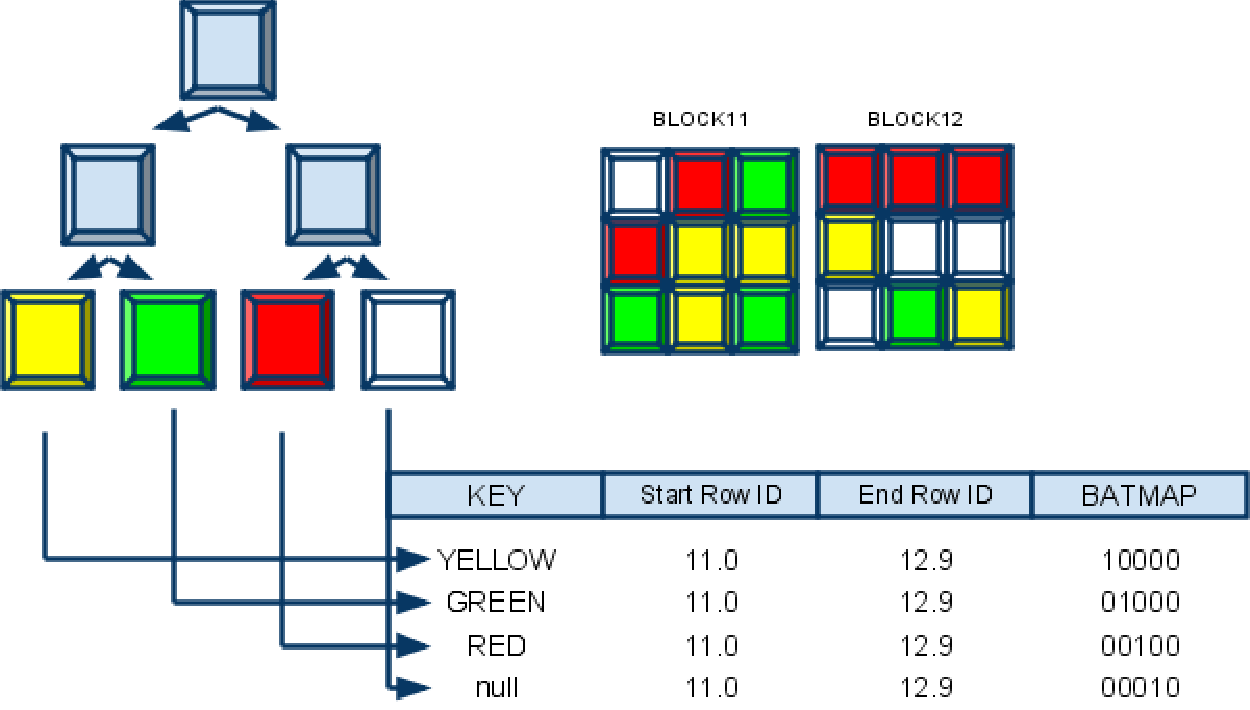
\includegraphics[width=1\textwidth]{bitmap_index.pdf}}
  \caption{Битовый индекс}
  \label{fig:bitmap_index}
\end{figure}

Сильные стороны:

\begin{itemize}
  \item компактность представления (занимает мало места);
  \item быстрое чтение и поиск по предикату <<равно>>;
\end{itemize}

Слабые стороны:

\begin{itemize}
  \item невозможность изменить способ кодирования значений в процессе обновления данных;
\end{itemize}

У PostgreSQL нет возможности создать постоянный битовый индекс, но база может на лету создавать данные индексы для объединения разных индексов. Чтобы объединить несколько индексов, база сканирует каждый необходимый индекс и готовит битовую карта в памяти с расположением строк таблицы. Битовые карты затем обрабатываются AND/OR операцией по мере требования запроса и после этого выбираются колонки с данными.



\subsection{GiST индекс}

GiST (Generalized Search Tree)~--- обобщение B-Tree, R-Tree дерево поиска по произвольному предикату. Структура дерева не меняется, по прежнему в каждом не листовом узле хранятся пары (Значения, Номер страницы), а количество детей совпадает с количеством пар в узле. Существенное отличие состоит в организации ключа. B-Tree деревья заточены под поиск диапазонов, и хранят максимумы поддерева-ребёнка. R-Tree~--- региона на координатной плоскости. GiST предлагает в качестве значений в не листовых узлах хранить ту информацию, которую мы считаем существенной, и которая позволит определить, есть ли интересующие нас значения (удовлетворяющие предикату) в поддереве-ребёнке. Конкретный вид хранимой информации зависит от вида поиска, который мы желаем проводить. Таким образом параметризовав R-Tree и B-Tree дерево предикатами и значениями мы автоматически получаем специализированный под задачу индекс (PostGiST, pg\_trgm, hstore, ltree, прочее).

Сильные стороны:

\begin{itemize}
  \item эффективный поиск;
\end{itemize}

Слабые стороны:

\begin{itemize}
  \item большая избыточность;
  \item необходимость специализированной реализации под каждую группу запросов;
\end{itemize}

Остальные плюсы-минусы совпадают с B-Tree и R-Tree индексами.



\subsection{GIN индекс}

GIN (Generalized Inverted Index)~--- обратный индекс, используемым полнотекстовым поиском PostgreSQL. Это означает, что в структуре индексов с каждой лексемой сопоставляется отсортированный список номеров документов, в которых она встречается. Очевидно, что поиск по такой структуре намного эффективнее, чем при использовании GiST, однако процесс добавления нового документа достаточно длителен.



\subsection{Cluster индекс}

Не является индексом, поскольку производит кластеризацию таблицы по заданному индексу. Более подробно можно почитать в разделе <<\ref{sec:hard-drive-cluster}~\nameref{sec:hard-drive-cluster}>>.



\subsection{BRIN индекс}

Версия PostgreSQL 9.5 привнесла с собой новый вид индексов~--- BRIN (Block Range Index, или индекс блоковых зон).

\begin{figure}[ht!]
  \center{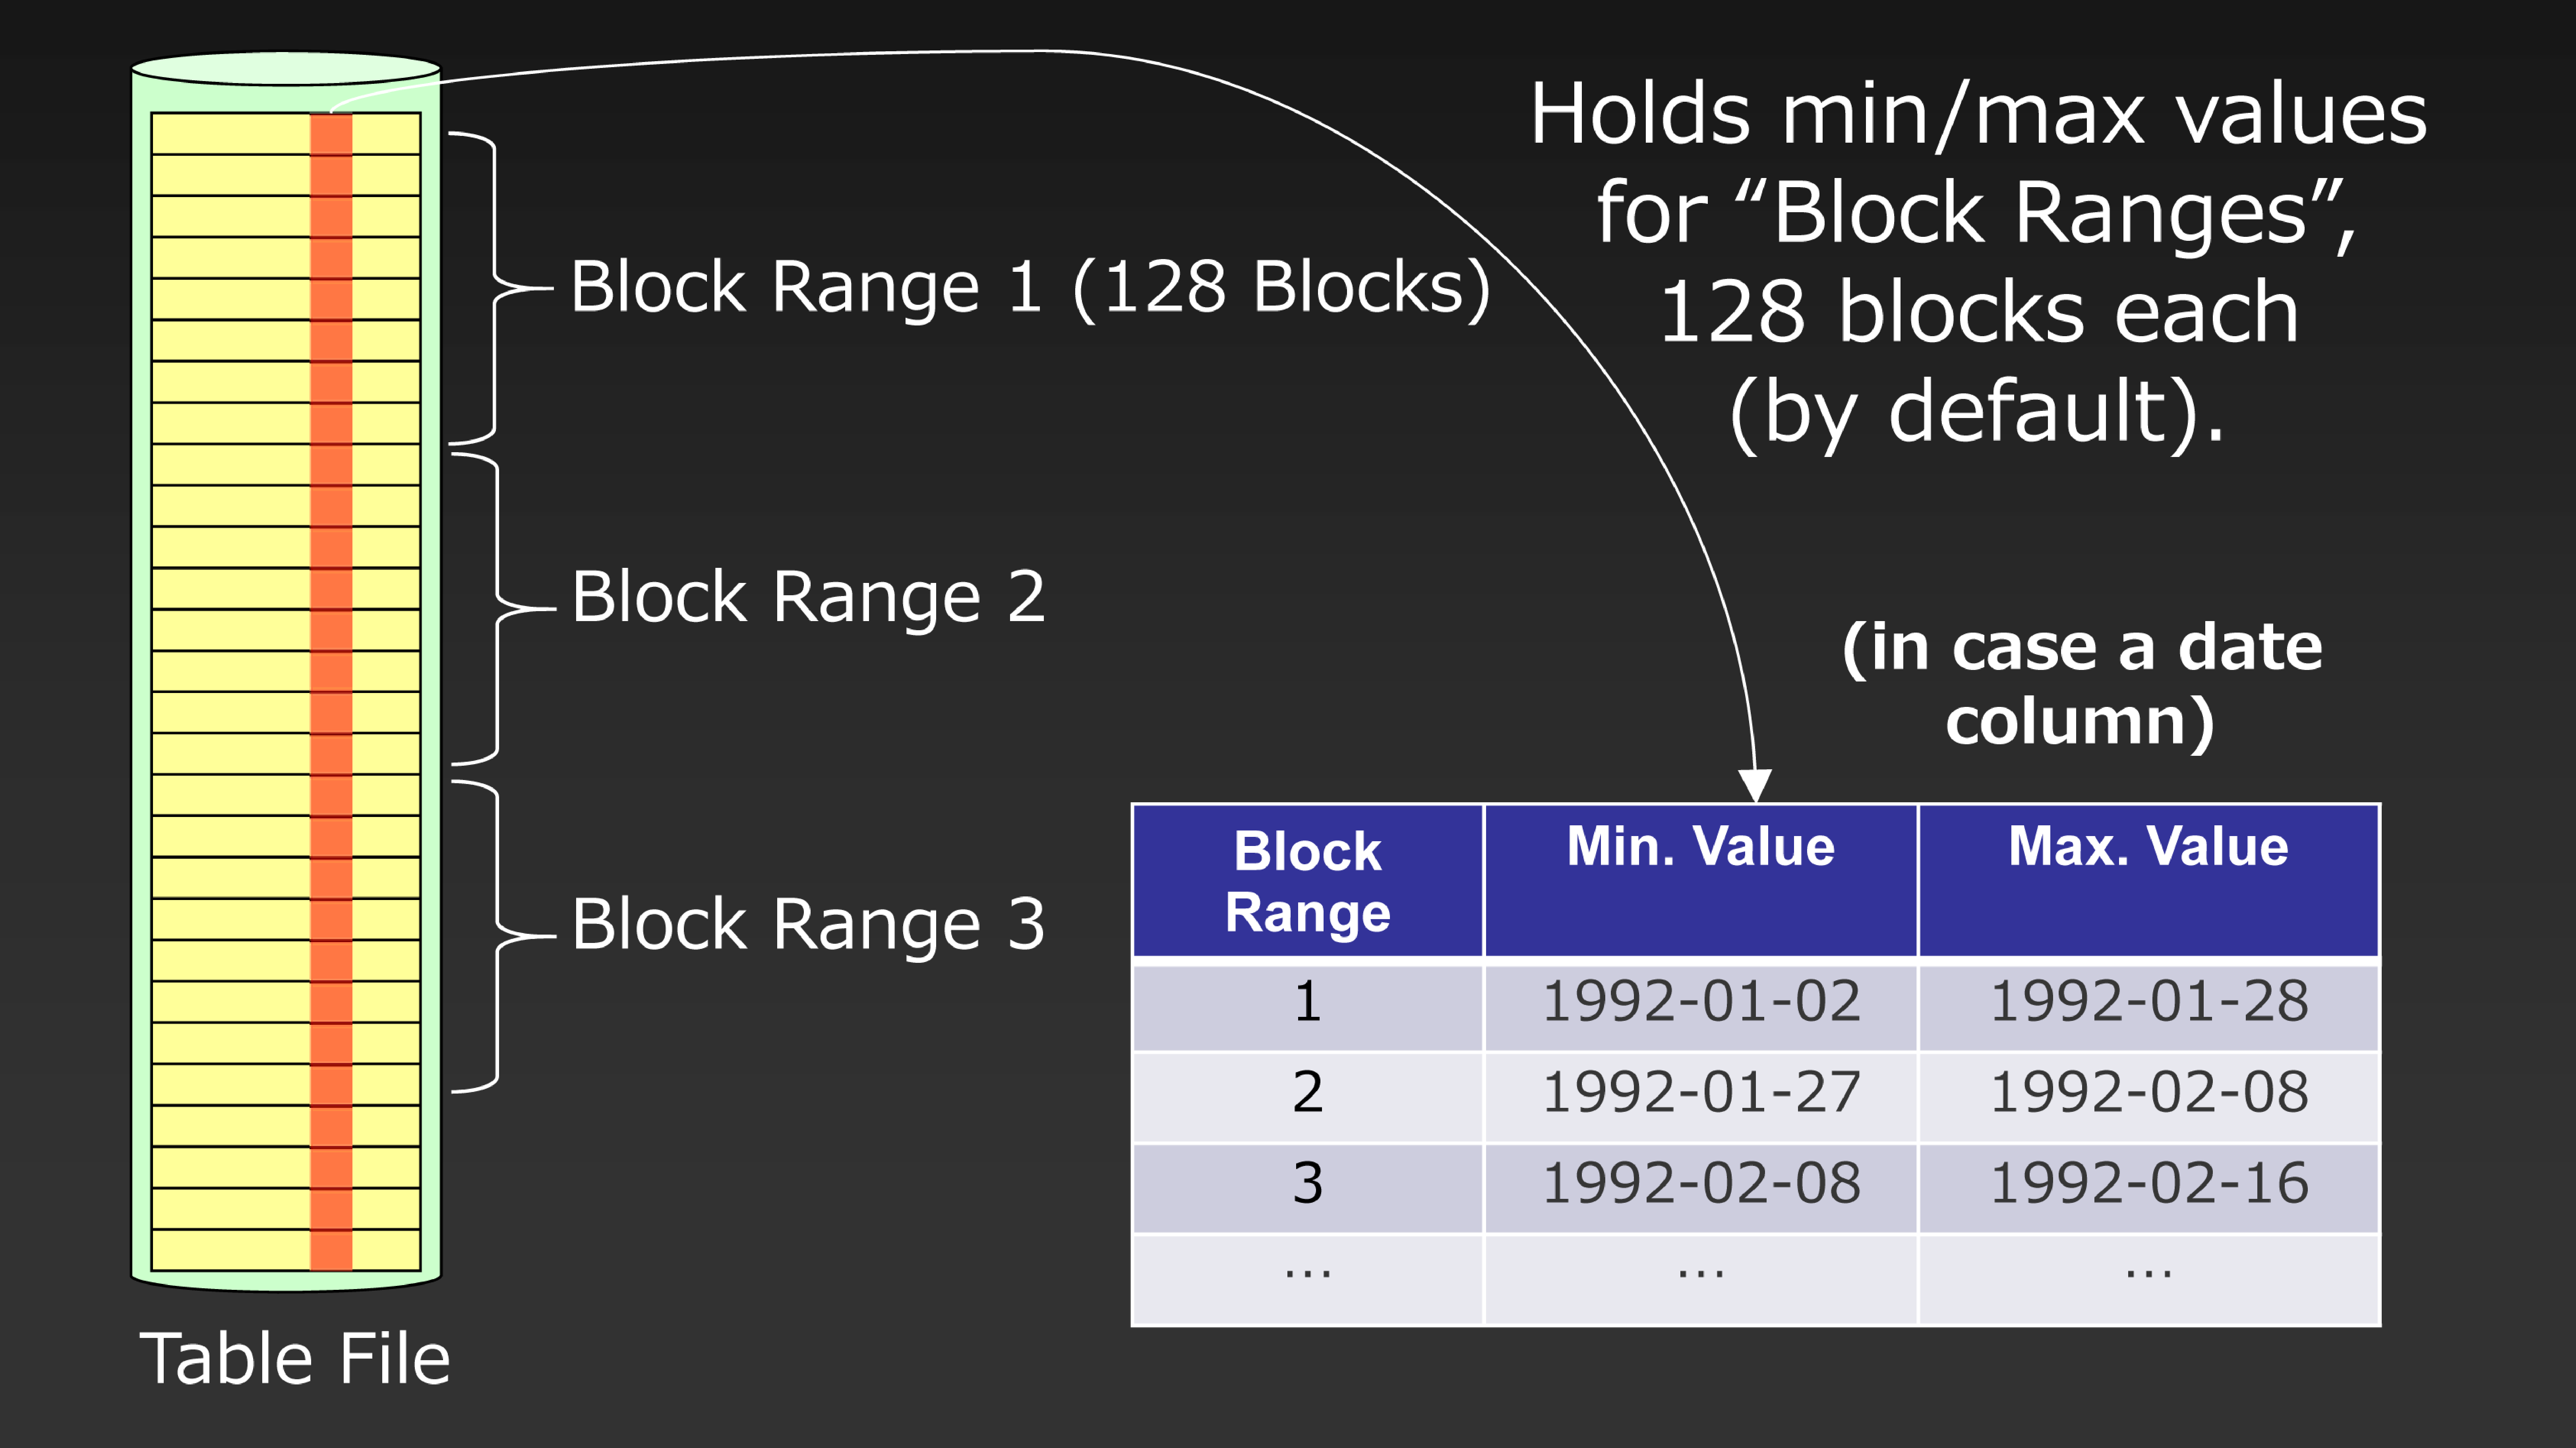
\includegraphics[width=1\textwidth]{brin_index.pdf}}
  \caption{BRIN индекс}
  \label{fig:brin_index}
\end{figure}

В отличие от привычного B-Tree, этот индекс намного эффективнее для очень больших таблиц, и в некоторых ситуациях позволяет заменить собой партицирование (подробно можно почитать в разделе <<\ref{sec:partitioning}~\nameref{sec:partitioning}>>). BRIN-индекс имеет смысл применять для таблиц, в которых часть данных уже по своей природе как-то отсортирована. Например, это характерно для логов или для истории заказов магазина, которые пишутся последовательно, а потому уже на физическом уровне упорядочены по дате/номеру, и в то же время таблицы с такими данными обычно разрастаются до гигантских размеров.

Под блоковой зоной (Block Range) подразумевается набор страниц, физически расположенных по соседству в таблице. Для каждой такой зоны создается некий идентификатор, отвечающий за <<место>> этой зоны в таблице. Для лога это может быть дата создания записи. Поиск по такому индексу осуществляется с потерями информации, то есть выбираются все записи, входящие в блоковые зоны с идентификаторами, соответствующими запросу, но среди записей в этих зонах могут попадаться такие, которые на следующем этапе надо будет отфильтровать. Размер индекса при этом очень маленький, и он почти не нагружает базу. Размер индекса обратно пропорционален параметру \lstinline!pages_per_range!, отвечающему за количество страниц на зону. В то же время, чем меньше размер зоны, тем меньше <<лишних>> данных попадёт в результат поиска (надо подходить к этому параметру с умом).

Индексы BRIN могут иметь один из нескольких встроенных классов операторов, по которым будет осуществляться разбивка на зоны и присвоение идентификаторов. Например, \lstinline!int8_minmax_ops! применяется для операций сравнения целых чисел, а \lstinline!date_minmax_ops! для сравнения дат.



\section{Возможности индексов}


\subsection{Функциональный индекс (functional index)}

Вы можете построить индекс не только по полю/нескольким полям таблицы, но и по выражению, зависящему от полей. Пусть, например, в вашей таблице foo есть поле \lstinline!foo_name!, и выборки часто делаются по условию <<первая буква из поля foo\_name в любом регистре>>. Вы можете создать индекс

\begin{lstlisting}[language=SQL,label=lst:summary-indexes1,caption=Индекс]
CREATE INDEX foo_name_first_idx ON foo ((lower(substr(foo_name, 1, 1))));
\end{lstlisting}

и запрос вида

\begin{lstlisting}[language=SQL,label=lst:summary-indexes2,caption=Запрос]
SELECT * FROM foo WHERE lower(substr(foo_name, 1, 1)) = 'а';
\end{lstlisting}

будет его использовать.



\subsection{Частичный индекс (partial index)}

Под частичным индексом понимается индекс с предикатом WHERE. Пусть, например, у вас есть в базе таблица \lstinline!scheta! с параметром \lstinline!uplocheno! типа boolean. Записей, где \lstinline!uplocheno = false! меньше, чем записей с \lstinline!uplocheno = true!, а запросы по ним выполняются значительно чаще. Вы можете создать индекс

\begin{lstlisting}[language=SQL,label=lst:summary-indexes3,caption=Индекс]
CREATE INDEX scheta_neuplocheno ON scheta (id) WHERE NOT uplocheno;
\end{lstlisting}

который будет использоваться запросом вида

\begin{lstlisting}[language=SQL,label=lst:summary-indexes4,caption=Запрос]
SELECT * FROM scheta WHERE NOT uplocheno AND ...;
\end{lstlisting}

Достоинство подхода в том, что записи, не удовлетворяющие условию WHERE, просто не попадут в индекс.


\subsection{Уникальный индекс (unique index)}

Уникальный индекс гарантирует, что таблица не будет иметь более чем одну строку с тем же значением. Это удобно по двум причинам: целостность данных и производительность. Поиск данных с использованием уникального индекса, как правило, очень быстрый.


\subsection{Индекс нескольких столбцов (multi-column index)}

В PostgreSQL возможно создавать индексы на несколько столбцов, но нам главное нужно понять когда имеет смысл создавать такой индекс, поскольку планировщик запросов PostgreSQL может комбинировать и использовать несколько индексов в запросе путем создания битового индекса (<<\ref{sec:indexes-bitmap-index}~\nameref{sec:indexes-bitmap-index}>>). Можно конечно создать индексы, которые охватять все возможные запросы, но за это придется платить производительностью (индексы нужно перестраивать при запросах на модификацию данных). Нужно также помнить, что индексы на несколько столбцов могут использоваться только запросами, которые ссылаются на эти столбцы в индексе в том же порядке. Индекс по столбцам \lstinline!(a, b)! может быть использован в запросах, которые содержат \lstinline!a = x and b = y! или \lstinline!a = x!, но не будет использоваться в запросе вида \lstinline!b = y!. Если это подходит под запросы вашего приложения, то данный индекс может быть полезен. В таком случае создание индекса на поле \lstinline!a! было бы излишним. Индексы нескольких столбцов с указанием уникальности (\lstinline!unique!) может быть также полезен для сохранения целосности данных (т.е. когда набор данных в этих стобцах должен быть уникальным).
